\item \textbf{{[}ALVL/9597/2015/P2/Q1{]} }

The management of a university is keen to implement changes which
will result in higher student attainment. The management believes
this is possible if it collects more data about its students which
is then analysed.

Possible data that might be collected includes: assignment grades,
books taken out of the library, attendance at lectures, attendance
at tutorials, meetings with personal tutor, email exchanges with university
staff. and participation in sporting and cultural activities.

University staff are classified as either academic or management.
All data about students will be available to academic staff for viewing
and editing. Summary information, which does not identify any individual
student. will be viewable by some management staff. Students have
no access to the data.

A project working party is to be set up consisting of representatives
from across the university. The working party will define the scope
of the project. It will consider what data is to be collected. it
will also decide what the data is to be used for and consider any
potential further use of the data.

If this project has a successful outcome, the university will market
its expertise to other universities. 
\begin{enumerate}
\item Give \textbf{three} different representative members of the working
party. Justify each choice. \hfill{}{[}6{]}
\item The working party has been asked to produce a list of issues that
will be considered by the Ethics Committee of the university.

State \textbf{two} issues that could be on the list.\hfill{} {[}2{]}
\end{enumerate}
After consideration of the reports from the working party and the
Ethics Committee the university management decide to proceed with
the project. A project team is put together to design and implement
a new software system.

The initial work of the project team involves an investigation process. 
\begin{enumerate}
\item[(c)] Name \textbf{two }techniques that can be used by the project team
in the investigation process. For each technique, explain how it can
be used in this project.\hfill{} {[}6{]}
\item[(d)] A detailed report is produced following the investigation.Thls report
will form the starting point of the design stage. Describe \textbf{two}
sections of the report.\hfill{} {[}4{]}
\end{enumerate}
The project team draw up a list of activities that will be required
for the completion of the software project:
\begin{center}
\begin{tabular}{|c|l|c|}
\hline 
Activity & \texttt{\hspace{0.01\columnwidth}}Activity Description  & Expected Duration (in weeks)\tabularnewline
\hline 
A & Design solution to project & 10\tabularnewline
\hline 
B & Development of solution to project & 25\tabularnewline
\hline 
C & Produce documentation & 12\tabularnewline
\hline 
D & Testing & 30\tabularnewline
\hline 
E & implement system & 8\tabularnewline
\hline 
F & Acceptance trials & 2\tabularnewline
\hline 
\end{tabular}
\par\end{center}

A first attempt to produce a Program Evaluation and Review Technique
(PERT) chart from the activity table is: 
\begin{center}
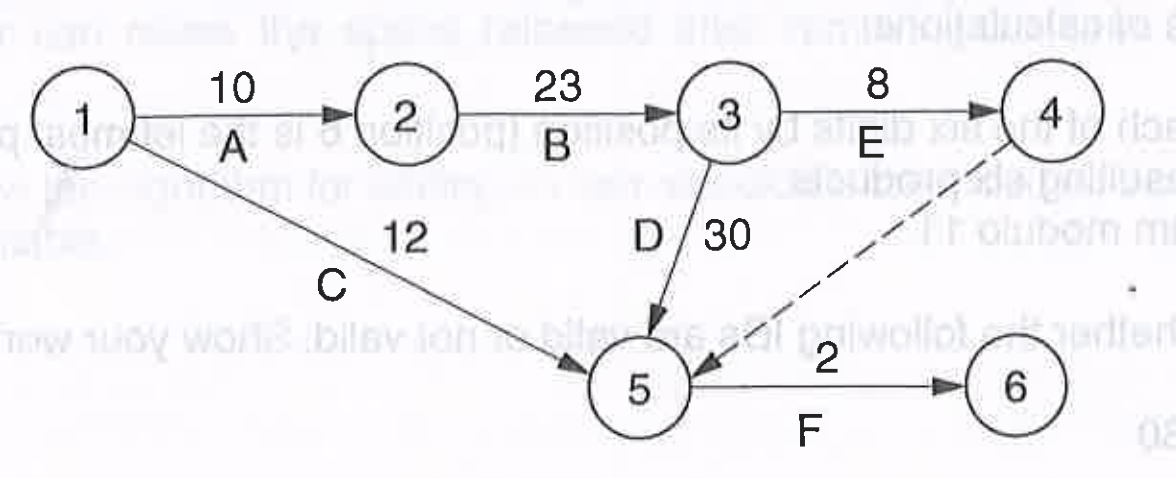
\includegraphics[width=0.5\paperwidth]{C:/Users/Admin/Desktop/Github/question_bank/LyX/static/img/9597-ALVL-2015-P2-Q1}
\par\end{center}
\begin{enumerate}
\item[(e)] {}
\begin{enumerate}
\item Describe \textbf{two} benefits that can be gained by producing a PERT
chart from the activity table. \hfill{}{[}2{]}
\item Explain the significance of the dashed line on the PERT chart. \hfill{}{[}2{]}
\item There are two errors on the PERT chart. identify these errors. Redraw
the PERT chart to show the changes needed to correct these errors.
\hfill{}{[}2{]}
\end{enumerate}
\item[(f)]  Using your PERT chart from part \textbf{(e)(iii)}: 
\begin{itemize}
\item State the minimum time in which the project could be completed.\hfill{}
{[}1{]}
\item By how many weeks can the start of the production of documentation
be delayed without delaying the whole project? \hfill{}{[}1{]}
\item Describe and give an example of concurrent activities.\hfill{} {[}2{]}
\item Describe and give an example of dependent activities. \hfill{}{[}2{]}
\end{itemize}
\end{enumerate}
Output from the system is made available to permitted staff via the
university intranet. However, the university intranet can be accessed
by all students and staff. both locally and remotely, via the lnternet.
The system needs security measures to prevent all types of unauthorised
access. 
\begin{enumerate}
\item[(g)]  Describe\textbf{ two} suitable physical security measures that could
be adopted. \hfill{}{[}4{]}
\item[(h)]  Describe \textbf{two} suitable software security measures that could
be adopted. \hfill{}{[}4{]}
\end{enumerate}
Following the success of the project, management decides that the
software system will be marketed to other universities. 
\begin{enumerate}
\item[(i)]  Explain how the university's investment in the software can be legally
protected. \hfill{}{[}2{]}
\end{enumerate}